\documentclass[10pt]{beamer}



%%%
% PREAMBLE FOR THIS DOC 
%%%
%https://tex.stackexchange.com/questions/68821/is-it-possible-to-create-a-latex-preamble-header
\usepackage{/Users/miw267/Repos/csci246_spring2025/slides/preambles/beamer_preamble_for_CSCI246}

\usepackage{wrapfig}  


%%% TRY TO RESHOW TOC AT EACH SECTION START (with current section highlighted)
% Reference: https://tex.stackexchange.com/questions/280436/how-to-highlight-a-specific-section-in-beamer-toc
\newcommand\tocforsect[2]{%
  \begingroup
  \edef\safesection{\thesection}
  \setcounter{section}{#1}
  \tableofcontents[#2,currentsection]
  \setcounter{section}{\safesection}
  \endgroup
}


\usepackage[normalem]{ulem} % for strikeout (\sout)

%%%% HERES HOW TO DO IT CORRECTLY
% FIRST IN .STY FILE, DO
%\usetheme[sectionpage=none]{metropolis}
% THEN AT EACH SECTION DO
%\begin{frame}{Outline}
%  \tableofcontents[currentsection]	
%\end{frame}



%\setbeamertemplate{navigation symbols}{}
%\setbeamertemplate{footline}[frame number]{}


%%%
% DOCUMENT
%%%

\begin{document}

%\maketitle

%% Title page frame
%\begin{frame}
%    \titlepage 
%\end{frame}



\title{02/03/2026: Continuous Random Variables (Part 1)}
\author{CSCI 546: Diffusion Models}
\date{Textbook reference: Sec 4.1-4.5}

\begin{frame}
    \titlepage 
\end{frame}

\begin{frame}
%\begin{myyellowbox}[title=Opening Discussion ($\approx$ 5 mins)]
%Find a partner and discuss these questions.
%\begin{enumerate}
%	\item What is your early reflection on the class?
%		\begin{itemize}
%		\item[a)] goal
%		\item[b)] hope
%		\item[c)] fear
%		\item[d)] like
%		\item[e)] dislike
%		\end{itemize}
%	\item Reflect on your experience reading the textbook.
%\end{enumerate}
%\end{myyellowbox}
%\vfill 
%\pause 
\begin{mygreenbox}[title=Announcement (Sign-in Sheet)]
Please sign the sign-in sheet.
\end{mygreenbox}
%\vfill 
%\pause 
%\begin{myredbox}[title=\text{Announcement (Office Hours)}]
%My office hours today need to be changed due to a grant meeting.  If you would like to meet on today, please send me an email to set up a time.
%\end{myredbox}
%\vfill 
%\pause 
%\begin{myyellowbox}[title=\text{Announcement (Group exercises)}]
%Group exercises will be posted to the course repo after class. Please continue working on what you don't finish in class.  
%\end{myyellowbox}
\end{frame}

\begin{frame}[standout]
Review Problem Set \#5	
\end{frame}

\begin{frame}[standout]
Concepts for Problem Set \#6
\end{frame}


\begin{frame}{Continuous random variables}

\begin{mygreenbox}[title=Definition (GS Sec 4.1)]
A random variable $X$ is called \textbf{continuous} if its distribution function $F(x) = P(X \leq x)$ can be written as 
\[ F(x) = \int_{-\infty}^x f(u) \wrt{u} \]
for some integrable $f : \R \to [0,\infty)$.
\end{mygreenbox}
\vfill

\colorbox{red!30}{\textbf{Remark}.} If X is a random variable with probability density $f$ below

\begin{center}
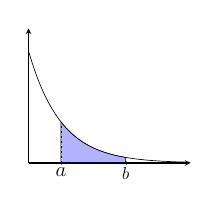
\begin{tikzpicture}[scale=0.3]
\begin{axis}[
    axis lines=middle,
    xlabel={},
    ylabel={},
    xmin=0, xmax=5,
    ymin=0, ymax=1.2,
    samples=200,
    axis line style={line width=2pt},
    xtick={1,3},
    xticklabels={\Huge $a$, \huge $b$},
    ytick=\empty,
]
% Curve
\addplot[thick, domain=0:5] {exp(-x)};

% Shaded area from a to b
\addplot[
    domain=1:3,
    fill=blue,
    fill opacity=0.3
] {exp(-x)} \closedcycle;

% Vertical lines at a and b
\addplot[dashed] coordinates {(1,0) (1,{exp(-1)})};
\addplot[dashed] coordinates {(3,0) (3,{exp(-3)})};

\end{axis}
\end{tikzpicture}
\end{center}
then 
\[ P(a \leq X \leq b) = \texttt{shaded area}\]
\end{frame}
	

\begin{frame}{Example: Exponential Distribution}

\begin{minipage}[c]{0.52\textwidth}
\begin{mygreenbox}[title=Definition]
A continuous random variable whose probability density function is given, for some $\lambda>0$, by
\begin{align*}
f(x) = \begin{cases}
\lambda e^{-\lambda x}, & \text{ if } x \geq 0  \\
0, & \text{ if } x < 0	 
\end{cases}
\end{align*}
is said to be an \textbf{exponential} random variable with parameter $\lambda$.
\end{mygreenbox}
\end{minipage}
\hfill
\begin{minipage}[c]{0.45\textwidth}
\centering
\includegraphics[width=\textwidth]{images/exponential_pdf}
\end{minipage}

\vfill 

\colorbox{red!30}{\textbf{Applications.}}
An exponential distribution often arises as the amount of time until some specific event occurs.  For example, the amount of time until...
\footnotesize 
\begin{itemize}
\item ... an earthquake occurs
\item ... a new war breaks out
\item ... you get a spam telephone call
\end{itemize}

\end{frame}

\begin{frame}{Memorylessness}

\begin{mygreenbox}[title=Definition]
We say that a non-negative random variable $X$ is \textbf{memoryless} if 
\begin{align}
P(X > s+t \mid X > t ) = P (X>s), \qquad \text{ for all } s,t \geq 0
\label{eqn:memoryless}
\end{align}


\end{mygreenbox}
\vfill 
\only<2>{\colorbox{yellow!30}{\textbf{Poll.}} Who can explain what the above equation is saying?}

\only<3-4>{\colorbox{red!30}{\textbf{Interpretation.}} If we think of $X$ as being the lifetime of some instrument, \Eqref{eqn:memoryless} says:

\vspace{.2cm}

\begin{quote}
\textit{If the instrument is alive at time $t$, the distribution of the remaining
amount of time that it survives is the same as the original lifetime distribution.}
\end{quote}
}



\only<4>{That is, it is as if the instrument does not ``remember'' that it has already been in use for time $t$.}


\end{frame}


\begin{frame}{Example: Uniform Distribution}

\begin{minipage}[c]{0.52\textwidth}
\begin{mygreenbox}[title=Definition]
A continuous random variable $X$ is said to be \textbf{uniform} on $[a,b]$ (or, equivalently, on $(a,b)$) if it has the probability density function
\begin{align*}
f(x) = \begin{cases}
\frac{1}{b-a}, & \text{ if } a < x < b  \\
0, & \text{ otherwise } 	 
\end{cases}
\end{align*}
\end{mygreenbox}
\end{minipage}
\hfill
\begin{minipage}[c]{0.45\textwidth}
\centering
\includegraphics[width=\textwidth]{images/uniform_pdf}
\end{minipage}


	
\vfill 

\colorbox{red!30}{\textbf{Applications.}}
Although simple, the uniform distribution is surprisingly useful.  E.g.:
\footnotesize 
\begin{itemize}
\item Random number generation by a computer.  (Non-uniform random numbers are often obtained by transforming uniform samples.)
\item Random angles in physics.
\item Monte carlo estimates of an integral $\int_{a}^b f(u) \wrt{u} \approx (b-a) \frac{1}{S} \sum_{s=1}^S f(u^^s)$ where $u^^s \sim U[a,b]$.
\end{itemize}

\end{frame}


\begin{frame}{Random Groups}

\begin{columns}
\begin{column}{0.33\textwidth}
Aubrey Williams: 7 \\ 
Austin Barton : 4 \\ 
Blake Sigmundstad: 3 \\ 
Diego Moylan: 3 \\ 
Dillon Shaffer: 2 \\ 
Ismoiljon Muzaffarov: 5 \\ 
Jacob Tanner: 8 \\\end{column}
\begin{column}{0.33\textwidth}
Josh Stoneback: 1 \\ 
Joshua Bowen: 2 \\ 
Joshua Culwell: 6 \\ 
Laura Banaszewski: 4 \\ 
Lina Hammel: 1 \\ 
Logan Racz: 8 \\\end{column}
\begin{column}{0.33\textwidth}
Matt Hall: 4 \\ 
Micah Miller: 2 \\ 
Mike Kadoshnikov: 1 \\ 
Owen Cool: 5 \\ 
Racquel Bowen: 6 \\ 
Samuel Mocabee: 7 \\ 
Tatiana Kirillova: 3 \\\end{column}
\end{columns}

\end{frame}



\begin{frame}{Group exercises - Problem Set 6}
\begin{enumerate}
\item (4.14.5b) Prove that the exponential distribution is memoryless.  (Note: the exponential distribution is the \textit{only} continuous distribution with this property!)
\item (4.5.5a) Let $X$ and $Y$ be independent continuous random variables.  Show that
\[ \E[g(X)h(Y)]= \E[g(X)] \E[h(Y)] \]
whenever these expectations exist.  If $X$ and $Y$ have the exponential distribution with parameter 1, find $\E[e^{\half (X+Y)}]$.
\item (4.5.4) Let $X$ and $Y$ be independent random variables each having the uniform distribution on $[0,1]$.  Let $U=\text{min}\set{X,Y}$ and  $V=\text{max}\set{X,Y}$.  Find $\E[U]$ and $\E[V]$, and then calculate $\Cov[U,V]$.   Are $U$ and $V$ independent? 
\end{enumerate}   
\end{frame}


\end{document}
